\documentclass[10pt,a4paper]{article}
\pdfinfoomitdate=1
\pdftrailerid{}
\pdfsuppressptexinfo=15

\usepackage[T1]{fontenc}
\usepackage[utf8]{inputenc}
\usepackage{lmodern}
\usepackage{microtype}
\usepackage[a4paper,margin=22mm]{geometry}
\usepackage{amsmath,amssymb}
\usepackage{booktabs,tabularx,array,longtable}
\usepackage{enumitem}
\usepackage{xcolor}
\usepackage{hyperref}
\usepackage{fancyhdr}
\usepackage{tikz}
\usetikzlibrary{arrows.meta,positioning,shapes.geometric,fit,calc}

\definecolor{navy}{HTML}{17324D}
\definecolor{teal}{HTML}{1B728C}
\definecolor{soft}{HTML}{F3F6F8}
\definecolor{warn}{HTML}{8A4B08}
\definecolor{greenish}{HTML}{2E6B57}
\hypersetup{
  colorlinks=true,
  linkcolor=navy,
  citecolor=teal,
  urlcolor=teal,
  pdftitle={Siamese Embedding Compression Research Program v0.3},
  pdfauthor={Guillaume Harbonnier},
  pdfsubject={Study 0 closure, Study 1B calibration, engineering benchmark design and pre-execution evidence controls},
  pdfkeywords={face verification, embedding compression, PCA, Siamese networks, non-inferiority, power, engineering benchmark, provenance, reproducibility}
}
\setlength{\parindent}{0pt}
\setlength{\parskip}{5pt}
\setlength{\emergencystretch}{1.5em}
\setlist[itemize,enumerate]{nosep,leftmargin=*}
\pagestyle{fancy}
\fancyhf{}
\fancyhead[L]{Siamese Embedding Compression Research Program}
\fancyhead[R]{v0.3 --- pre-execution synthesis}
\fancyfoot[C]{\thepage}
\renewcommand{\headrulewidth}{0.4pt}
\fancypagestyle{plain}{\fancyhf{}\fancyfoot[C]{\thepage}\renewcommand{\headrulewidth}{0pt}}

\newcommand{\fnmr}{\mathrm{FNMR}}
\newcommand{\fmr}{\mathrm{FMR}}
\newcommand{\DeltaFNMR}{\Delta_{\fnmr}}
\newcommand{\code}[1]{\texttt{#1}}

\title{\textbf{Siamese Embedding Compression Research Program}\\[4pt]
\large From corrected biometric uncertainty to engineering value and evidence-controlled execution}
\author{Guillaume Harbonnier\\
\small Independent exploratory research\\
\small \url{https://github.com/gharbonnier78/siamese-embedding-compression-lab}}
\date{Version 0.3 --- 15 September 2026}

\begin{document}
\maketitle
\thispagestyle{empty}

\begin{center}
\fcolorbox{warn}{soft}{\parbox{0.92\linewidth}{
\textbf{Scope and status.}
This document synchronizes the human-readable research narrative with the current repository state.
It reports no protected Study 1B SCREEN or qualification TEST outcome, opens no representation geometry,
activates no amendment, and does not authorize canonical Jungle Championship Phase A execution.
The normative authority remains the frozen protocol, review and Chronicle artifacts in the repository.
}}
\end{center}

\begin{abstract}
The programme investigates whether a face embedding can be compressed from 512 to 128 dimensions while
retaining decision-relevant biometric performance and producing enough engineering value to justify the
qualification burden. The initial controlled experiment, Study 0, compared raw512, random128, PCA128 and a
learned Siamese128 projection on a frozen ImageNet ResNet-18 representation. After an audit showed that the
original pair-level uncertainty treatment ignored repeated identity participation, the historical scores were
re-analysed with dependence-aware uncertainty. The corrected conclusion remained negative: preservation was
not demonstrated in the frozen experiment.

Study 1 changes the substrate and the evidence architecture before reopening the compression question.
Study 1A specifies qualification of a face-specific AdaFace R100 512D backbone. Study 1B retains a matched
raw/random/PCA/Siamese comparison but requires identity/template-aware uncertainty and prospective calibration
of the complete decision procedure. Two frozen synthetic calibration campaigns, S4N1 and S4N2, both failed to
attain the 90\% power target at the acceptable truth $\DeltaFNMR=0.01$; they remain closed negative and S4N3
has not been launched.

A distinct engineering workstream therefore asks a different question: what resource envelope does 512D to
128D compression create on a real edge 1:N platform? Structural arithmetic proves a 75\% vector-payload
reduction for equal encoding, but latency, throughput and energy must be measured. The Jungle Championship
benchmark contract defines that future measurement and surrounds it with D1--D3 evidence-firewall rules so
hardware, backend, threading and measurement choices cannot be silently tuned from target-workload previews.
The accepted v0.5 design closed D1--D3 while keeping execution inadmissible and construct validity unreviewed.
The prospective v0.6 hardening clarifies possession versus evidence-creation influence, separates mechanically
checkable temporal ordering from provenance claims, and evaluates informational overlap per lock-defining
choice. This version documents the full chain, the current blockers and the next admissible sequence.
\end{abstract}

\tableofcontents
\newpage

\section{Research question and programme decomposition}

The programme is intentionally split into scientific and engineering questions.

\begin{quote}
\textbf{Scientific preservation question:} can a 128D route remain sufficiently close to raw512 at a frozen
biometric operating point under a dependence-aware uncertainty procedure?
\end{quote}

\begin{quote}
\textbf{Engineering value question:} what memory, arithmetic, latency, throughput and energy consequences follow
from using 128D rather than 512D on a frozen target platform?
\end{quote}

A favorable engineering result cannot rescue a failed biometric qualification rule, and a favorable biometric
result would not by itself prove a useful edge-system benefit. The two evidence streams must remain distinct.

\begin{figure}[ht]
\centering
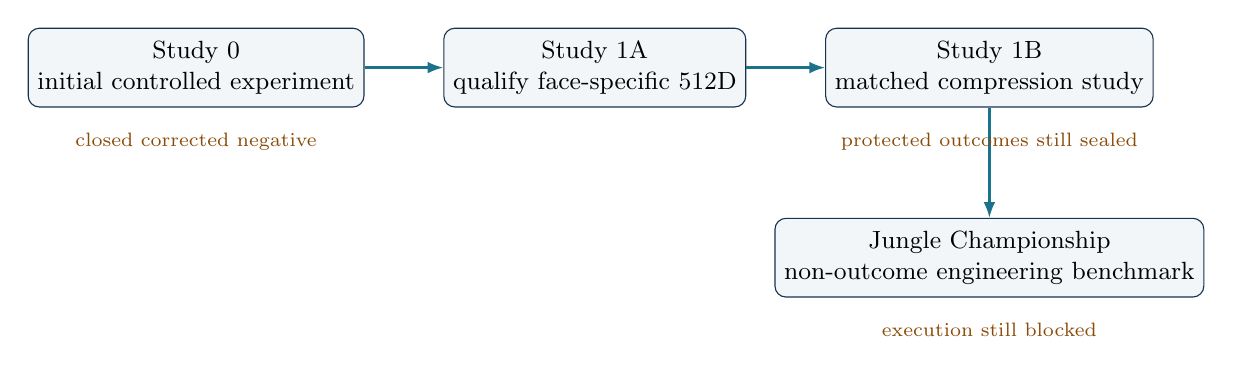
\begin{tikzpicture}[
node distance=7mm and 10mm,
box/.style={draw=navy,rounded corners,fill=soft,align=center,minimum width=33mm,minimum height=10mm,font=\small},
arr/.style={-{Latex[length=2mm]},thick,color=teal}
]
\node[box] (s0) {Study 0\\initial controlled experiment};
\node[box,right=of s0] (s1a) {Study 1A\\qualify face-specific 512D};
\node[box,right=of s1a] (s1b) {Study 1B\\matched compression study};
\node[box,below=14mm of s1b] (eng) {Jungle Championship\\non-outcome engineering benchmark};
\draw[arr] (s0)--(s1a);
\draw[arr] (s1a)--(s1b);
\draw[arr] (s1b)--(eng);
\node[font=\scriptsize,text=warn,below=2mm of s0] {closed corrected negative};
\node[font=\scriptsize,text=warn,below=2mm of s1b] {protected outcomes still sealed};
\node[font=\scriptsize,text=warn,below=2mm of eng] {execution still blocked};
\end{tikzpicture}
\caption{Programme decomposition. Engineering benchmarking is related to, but not a substitute for, scientific
qualification.}
\end{figure}

\section{Study 0: the corrected initial experiment}

Study 0 used a frozen ImageNet ResNet-18 512D representation on LFW. Four routes were compared:

\begin{itemize}
\item \textbf{raw512}: no dimensionality reduction;
\item \textbf{random128}: seeded random linear projection;
\item \textbf{PCA128}: unsupervised principal-component projection;
\item \textbf{Siamese128}: supervised shared linear 512-to-128 projection trained with contrastive loss.
\end{itemize}

The primary operating point was empirical $\fmr=0.01$ with a frozen non-inferiority margin
$\DeltaFNMR=0.03$, where
\[
\DeltaFNMR(m,\alpha)=\fnmr_m(\alpha)-\fnmr_{\mathrm{raw512}}(\alpha).
\]

A later audit found that the original uncertainty estimator resampled pair rows even though the same identity
can participate in several comparisons. The historical score bundle was preserved and re-analysed with a
subject-level dependence-aware procedure. The corrected result remained negative: random128, PCA128 and
Siamese128 all failed the frozen non-inferiority rule on all five seeds in the corrected Study 0 report.

The inference is deliberately bounded. Study 0 does not prove that 128D compression is universally inferior,
that PCA is unsuitable, or that metric learning is ineffective. It establishes only that preservation was not
demonstrated in this frozen experiment.

\section{Study 1A: qualify the source representation first}

Study 1A changes the source embedding before compression is reconsidered. The specified backbone is:

\begin{itemize}
\item AdaFace;
\item R100 / \code{ir\_101};
\item 512-dimensional output;
\item released WebFace12M-trained checkpoint;
\item frozen inference, with no face-backbone training inside Study 1A.
\end{itemize}

The evaluation hierarchy separates sanity/reproduction benchmarks from a preferred low-FMR primary endpoint.
LFW, CFP-FP, AgeDB-30, CALFW and CPLFW are useful reproduction challenges but are not treated as numerically
interchangeable with IJB-C. NIST FRTE is external evaluation context and is not silently substituted as local
qualification data.

Gate A is conjunctive: provenance and pipeline integrity, frozen reproduction thresholds and a low-FMR primary
endpoint. If lawful and replayable IJB-C access is unavailable, the low-FMR gate remains indeterminate until a
prospective amendment freezes a public/replayable replacement and its own reference criterion.

This v0.3 synthesis does not introduce a new Study 1A scientific result.

\section{Study 1B: matched compression study}

The Study 1B route catalog preserves the conceptual roles:

\begin{table}[ht]
\centering
\begin{tabularx}{\linewidth}{l X X}
\toprule
\textbf{Route} & \textbf{Purpose} & \textbf{Learning source}\\
\midrule
raw512 & reference representation & frozen face backbone\\
random128 & dimensionality-only control & seeded random matrix\\
PCA128 & unsupervised compression control & TRAIN only\\
Siamese128 & supervised metric-compression candidate & TRAIN pair supervision only\\
\bottomrule
\end{tabularx}
\end{table}

Real SCREEN, qualification TEST, real route performance and representation geometry remain unopened.
A method name, selector label or screening result cannot substitute for a protected qualification result.

\section{Dependence-aware uncertainty}

Biometric pair rows are not automatically independent evidence. If one identity contributes to several genuine
or impostor comparisons, resampling rows can understate uncertainty.

Study 1B therefore requires:

\begin{itemize}
\item identity/template/capture-level sampling units justified by the benchmark graph;
\item paired raw/candidate resampling draws;
\item separation of model/projection seeds from bootstrap Monte-Carlo seeds;
\item no interpretation of bootstrap replicate count as independent sample size;
\item frozen low-FMR threshold and degeneracy handling;
\item revalidation if the future trial graph materially changes.
\end{itemize}

The lesson is methodological: the uncertainty procedure is part of the decision system and must itself be
qualified before protected outcomes are interpreted.

\section{S4 calibration: two procedures, one synthetic population}

Before protected real outcomes can be used, Study 1B calibrated the complete frozen decision procedure on
known-truth synthetic worlds.

\subsection{S4N1}

S4N1 used the frozen identity-aware subject bootstrap. At true $\DeltaFNMR=0.01$, the prospectively preferred
selector achieved power 0.8690. The maximum observed selector power was 0.8695.

\subsection{S4N2}

S4N2 changed only the TEST uncertainty procedure to DAGJK20: 20 deterministic identity groups, delete-a-group
jackknife variance, and a one-sided Student-$t$ critical value
\[
t_{0.975,19}=2.0930240544.
\]
At true $\DeltaFNMR=0.01$, the prospectively preferred selector achieved power 0.8490. The maximum observed
selector power was 0.8535.

\begin{table}[ht]
\centering
\begin{tabular}{lrrr}
\toprule
 & \textbf{Fixed seed} & \textbf{Prospectively preferred} & \textbf{Observed maximum}\\
\midrule
S4N1 power at $\Delta=0.01$ & 0.8655 & 0.8690 & 0.8695\\
S4N2 power at $\Delta=0.01$ & 0.8470 & 0.8490 & 0.8535\\
\bottomrule
\end{tabular}
\caption{Archived synthetic power at the acceptable truth $\DeltaFNMR=0.01$.}
\end{table}

The two campaigns deliberately regenerated the same deterministic synthetic known-truth worlds. They are
\textbf{not} two independent validations of the generator. They are two uncertainty procedures on one synthetic
population.

Exact Clopper--Pearson Monte-Carlo intervals do not rescue the gate: the largest upper 95\% endpoint among the
$\Delta=0.01$ selector cells is 0.8797913, still below the frozen 0.90 target.

The admissible conclusion is therefore:
\begin{quote}
The frozen Study 1B decision procedures tested so far do not attain the preregistered 90\% power objective at
the acceptable synthetic truth $\DeltaFNMR=0.01$.
\end{quote}

S4N1 and S4N2 remain \code{CLOSED\_NEGATIVE}. S4N3 has not been launched. Continuing to introduce estimators
after observing each failure would create estimator-shopping risk unless a new prospective methodological
question independently motivates another procedure.

\section{Why the engineering benchmark still matters}

The S4 closure concerns the ability of a frozen qualification procedure to demonstrate non-inferiority.
It does not quantify the engineering value of a smaller vector.

For equal datatype and encoding, the dimensional ratio is exact:
\[
\frac{128}{512}=0.25.
\]
Therefore the vector payload falls by 75\%, and an exact dense dot-product numerator contains 75\% fewer
coordinate-wise contributions.

\begin{table}[ht]
\centering
\begin{tabular}{lrrr}
\toprule
\textbf{Representation} & \textbf{FP32} & \textbf{FP16} & \textbf{INT8}\\
\midrule
512D & 2,048 B & 1,024 B & 512 B\\
128D & 512 B & 256 B & 128 B\\
Saving & 1,536 B & 768 B & 384 B\\
\bottomrule
\end{tabular}
\caption{Structural per-template payload reduction.}
\end{table}

These are structural facts, not end-to-end benchmark results. They do not imply 4x lower latency or 75\%
lower energy.

\section{Jungle Championship: engineering scenario}

The Jungle Championship scenario models distributed autonomous edge units deployed at entrances, parking,
corridors, rooms and technical areas. A unit may perform local 1:N search, include RGB/NIR acquisition,
liveness/tamper functions, support intermittent connectivity and buffer events locally.

The workload model deliberately distinguishes:

\begin{itemize}
\item enrolled identities;
\item templates per identity;
\item passages or transactions;
\item image observations;
\item device count.
\end{itemize}

A stadium capacity is therefore not multiplied naively by camera count to invent a biometric gallery size or
comparison count.

For one planning scenario with 500,000 whitelist identities, 10,000 blacklist identities and three templates
per identity, the full gallery contains 1.53 million templates. At FP32:

\begin{itemize}
\item 512D payload: 3.13344 GB/device;
\item 128D payload: 0.78336 GB/device;
\item saving: 2.35008 GB/device.
\end{itemize}

The exact dense coordinate contributions per observation are 783.36 million at 512D versus 195.84 million at
128D. Across 50 fully replicated devices, aggregate gallery payload is 156.672 GB versus 39.168 GB.

A 25\% local-replication variant yields 0.82944 GB versus 0.20736 GB per device.

These numbers are deterministic workload arithmetic under stated assumptions. They are not measured timing
or energy results.

\section{Phase A: what the future benchmark is meant to measure}

Canonical Phase A is intended to measure exact dense 1:N search on a frozen target edge platform. The result
provenance must preserve at least:

\begin{itemize}
\item raw latency samples;
\item throughput;
\item RAM residency and swap behavior;
\item raw external power samples;
\item prospectively defined energy accounting, such as joules per identification;
\item temperature/throttling evidence when available;
\item complete backend, BLAS, threading, affinity and runtime state;
\item failure and exclusion logs.
\end{itemize}

The canonical power plane is external device-input or wall measurement. On-chip telemetry is supporting
diagnostic evidence only. The load generator is off-device so workload generation does not silently contaminate
the device-under-test measurements.

No target-workload pilot, smoke test, preview, capacity check, tuning pass or similar run may be used to choose
lock-defining settings before the execution-specific lock is frozen.

\section{D1--D3: evidence firewall for benchmark design}

The benchmark can be biased before any result is recorded if earlier measurements influence which hardware,
backend, thread count or measurement method is selected. D1--D3 address this design-stage leakage.

\subsection{D1: accountable provenance and attestation}

D1 applies to evidence whose creation or framing was influenced by the attesting party: produced, commissioned,
requested, specified, directed or materially framed. D1 also remains the completeness backstop for every
lock-defining choice.

\subsection{D2: bounded public temporal ordering}

For genuinely external or pre-existing evidence, D2 contributes one mechanically checkable fact: its timestamp
can be shown to predate the immutable repository-root public-information bound.

The accepted conservative anchor is:

\begin{itemize}
\item repository root commit \code{4b40e7254bff1b88a44d13fb55b366bc7d3fc263};
\item timestamp 2026-08-07T08:23:56Z;
\item root artifact \code{README.md}.
\end{itemize}

Only the temporal ordering is mechanically checkable from repository history. Source independence and absence
of attester influence are provenance claims and remain subject to accountable attestation.

\subsection{D3: classify information, not intention}

Prior evidence is classified by whether it can inform a lock-defining choice, not by a declared intention to
use or ignore it. Uncertainty defaults to informative.

The prospective v0.6 refinement makes overlap choice-specific:

\begin{itemize}
\item hardware class matters for platform-specific choices;
\item backend/BLAS evidence can transfer across hardware classes;
\item threading/affinity evidence can transfer across materially comparable execution models;
\item measurement-method evidence can transfer even across different hardware, dimensions or search families.
\end{itemize}

\section{v0.5 acceptance and v0.6 semantic hardening}

The focused independent review of v0.5 returned \textbf{ACCEPT}. It recorded:

\begin{itemize}
\item D2 closed;
\item D1/D2 responsibility split accepted;
\item repository-root public-information bound accepted;
\item prior D1--D3 design conditions satisfied;
\item canonical execution still inadmissible;
\item construct validity not reviewed.
\end{itemize}

The review also recorded three non-blocking items that must be closed before an execution-specific lock is
frozen:

\begin{description}
\item[N4.] The old D2 disqualifier list conflated influence over evidence creation/framing with mere possession,
receipt, citation or review.
\item[N5.] The phrase ``structural impossibility'' risked implying that the whole D2 mechanism was objective,
although only timestamp ordering is mechanically checkable.
\item[R1/N2.] A global hardware-class conjunction under-classified prior evidence relevant to portable backend/BLAS,
threading/affinity and measurement-method choices.
\end{description}

Environment-lock v0.6 corrects these prospectively without rewriting the accepted historical artifacts.
A fourth item, N6, hardens review transport: future packages ship exact normative artifacts and expected Git blob
SHA-1 values so reviewers can recompute Git object identity locally.

At the date of this document, v0.6 still awaits focused independent semantic re-review.

\section{Structural, measured and extrapolated claims}

The programme distinguishes three claim classes.

\begin{description}
\item[Structural.] Exact consequences of representation dimension and datatype, such as a 75\% payload reduction.
\item[Measured.] Observations produced on a frozen and reviewable execution environment, such as latency or wall-power samples.
\item[Extrapolated.] Calculations based on structural or measured quantities plus declared workload assumptions, such as
fleet-level memory or battery-life projections.
\end{description}

An extrapolation must not be restated as a measurement. Likewise, passing CI or engineering assurance is not a
scientific result.

\section{Current state as of 15 September 2026}

\subsection*{Closed and preserved}

\begin{itemize}
\item Study 0 corrected initial experiment: bounded negative closure.
\item S4N1: \code{CLOSED\_NEGATIVE}.
\item S4N2: \code{CLOSED\_NEGATIVE}.
\item S4N3: not launched.
\item D1, D2 and D3: accepted in the v0.5 history.
\item Repository-root temporal bound: accepted.
\item Protected SCREEN, qualification TEST, real-route performance and representation geometry: unopened.
\end{itemize}

\subsection*{Prospectively hardened, awaiting independent re-review}

\begin{itemize}
\item N4 possession-versus-influence semantics;
\item N5 objective-versus-attested wording;
\item R1/N2 choice-specific portable-information classification;
\item N6 self-contained review-package transport.
\end{itemize}

\subsection*{Still not materialized}

\begin{itemize}
\item target edge hardware;
\item external power meter;
\item off-device load generator;
\item complete configuration-choice provenance;
\item accountable provenance attestation;
\item frozen synthetic generator code identity;
\item execution-specific materialized environment lock;
\item construct-validity review.
\end{itemize}

Canonical Phase A execution is therefore \textbf{NOT ADMISSIBLE}.

Five bounded workflows are green on the current v0.6-bound head: CI, Research assurance, Engineering Assurance,
Non-outcome Preflight and Power Design Diagnostic. These are technical/repository assurance only. They are not
independent semantic acceptance of v0.6, construct validity, scientific evidence, platform binding or execution
authorization.

\section{Next admissible sequence}

The next sequence is deliberately ordered:

\begin{enumerate}
\item synchronize the human-facing narrative and monograph with the v0.6 contract;
\item freeze an immutable review basis once that documentation head is green;
\item build the N6-compliant self-contained focused review package;
\item obtain independent review of N4, N5 and R1/N2;
\item if accepted, conduct a separate construct-validity review of Phase A;
\item only then select and freeze real hardware, power meter, load generator and configuration provenance;
\item rerun bounded assurance on the exact execution head;
\item only after all execution gates are satisfied may canonical Phase A become eligible.
\end{enumerate}

None of these steps opens protected Study 1B biometric outcomes.

\section{Pedagogical interpretation}

Several reusable lessons emerge.

\begin{itemize}
\item \textbf{A negative result can improve the programme.} Study 0 and S4 did not produce the hoped-for qualification,
but they exposed weaknesses in uncertainty treatment and power.
\item \textbf{The measurement procedure is part of the system under qualification.} Bootstrap, jackknife, selector
semantics and low-FMR thresholding are not afterthoughts.
\item \textbf{Engineering value and scientific validity are different axes.} A 75\% structural payload reduction can be
real even while biometric preservation is not demonstrated.
\item \textbf{Prospective design must protect against information leakage before execution.} Target-workload previews can
bias hardware or runtime choices even when protected scientific outcomes remain unopened.
\item \textbf{Reviewability is an engineering property.} A package that cannot be independently inspected and byte-verified
is weaker even if its author-side checks pass.
\end{itemize}

\section{Authoritative artifact index}

This document is explanatory. The normative source of truth remains the repository.

\begin{itemize}
\item \code{AGENTS.md}
\item \code{harness-adoption.yaml}
\item \code{paper/study0\_v0.2.3.tex}
\item \code{paper/study1\_protocol\_v0.3-preexecution.md}
\item \code{protocol/decisions/STUDY1B\_S4N1\_S4N2\_SHARED\_POPULATION\_AND\_T19\_CLARIFICATION\_2026-09-08.yaml}
\item \code{protocol/benchmarks/STUDY1B\_JUNGLE\_CHAMPIONSHIP\_ENGINEERING\_BENCHMARK\_V0\_3\_2026-09-08.yaml}
\item \code{protocol/benchmarks/STUDY1B\_JUNGLE\_CHAMPIONSHIP\_ENGINEERING\_BENCHMARK\_V0\_3\_D1\_D3\_ADDENDUM\_V0\_2\_2026-09-14.yaml}
\item \code{protocol/benchmarks/STUDY1B\_JUNGLE\_CHAMPIONSHIP\_ENGINEERING\_ENVIRONMENT\_LOCK\_V0\_6\_2026-09-14.yaml}
\item \code{protocol/reviews/PR50\_CB124244\_D2\_V05\_FOCUSED\_REREVIEW\_VERDICT\_2026-09-10.md}
\item \code{protocol/chronicle/STUDY1B\_PR50\_PREEXECUTION\_SEMANTIC\_HARDENING\_V0\_6\_OPEN\_2026-09-14.yaml}
\end{itemize}

The repository is pinned to \code{scientific-research-harness} commit
\code{3b109adcdd9a8cba4df029d3803ee0e5cb5bdf98}.

\vfill
\begin{center}
\small
\textit{Interpretive rule: this monograph may summarize, teach and navigate the programme. It does not supersede
frozen protocols, independent-review verdicts or append-only Chronicle entries.}
\end{center}

\end{document}
